% *********************************************************************
% © 2026 Jeremy Sylvestre
%
% Permission is granted to copy, distribute and/or modify this document
% under the terms of the GNU Free Documentation License, Version 1.3 or
% any later version published by the Free Software Foundation; with no
% Invariant Sections, no Front-Cover Texts, and no Back-Cover Texts. A
% copy of the license is included in the appendix entitled “GNU Free
% Documentation License” that appears in the output document of this
% PreTeXt source code. All trademarks™ are the registered® marks of
% their respective owners.
%
% *********************************************************************
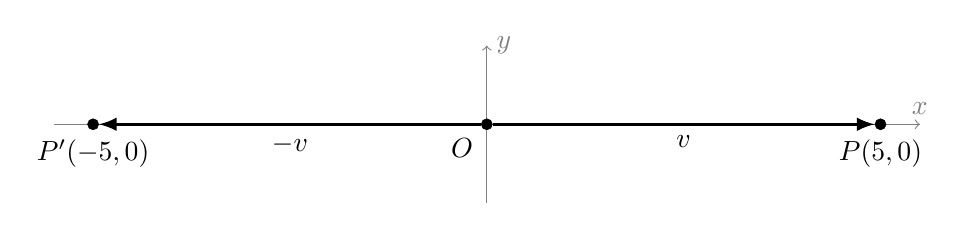
\begin{tikzpicture}[
	point/.style={circle,draw,very thin,fill,inner sep=0pt,minimum size=4pt},
	vector/.style={-latex,very thick},
	% scale=0.5
]
	\draw[gray,->] (-5.5,0) to (5.5,0) node[above] {$x$};
	\draw[gray,->] (0,-1) to (0,1) node[right] {$y$};

	\node[point] at (0,0) (o) [label=below left:$O$] {};
	\node[point] at (5,0) (p) [label=below:{$P(5,0)$}] {};
	\draw[vector] (o) to node[below] {$\uvec{v}$} (p);
	\node[point] at (-5,0) (pp) [label=below:{$P'(-5,0)$}] {};
	\draw[vector] (o) to node[below] {$- \uvec{v}$} (pp);

\end{tikzpicture}
